\documentclass{beamer}
\usetheme{Madrid}
\usepackage[T1]{fontenc}
\usepackage{mathpazo}
\usepackage{graphicx}
\usepackage{booktabs}
\usepackage{tikz}
\usetikzlibrary{positioning,arrows.meta,shapes.geometric,fit,backgrounds,calc}
\definecolor{cetnavy}{RGB}{10,26,63}
\definecolor{cetlight}{RGB}{225,231,242}
\setbeamercolor{structure}{fg=cetnavy}
\setbeamercolor{frametitle}{bg=cetnavy,fg=white}
\setbeamercolor{title}{bg=cetnavy,fg=white}
\setbeamertemplate{navigation symbols}{}
% =====================================================================
%  EDIT YOUR DETAILS HERE — this ONE file feeds every abstract & deck.
%  (Change a value, recompile; all 36 documents update.)
% =====================================================================
\newcommand{\seminarName}{Aflah Muhammed P}      % <-- your full name (guessed from your email; please verify)
\newcommand{\seminarRoll}{TVE00CS000}            % <-- your university register/roll number
\newcommand{\seminarClassRoll}{00}               % <-- your class roll no (the short one)
\newcommand{\seminarGuide}{Prof.\ <Guide Name>}  % <-- your guide
\newcommand{\seminarDept}{Department of Computer Science and Engineering}
\newcommand{\seminarCollege}{College of Engineering Trivandrum}
\newcommand{\seminarShortCollege}{CET}           % shown in the slide footer, e.g. "Aflah Muhammed P (CET)"
\newcommand{\seminarShortTitle}{B.Tech Seminar}  % middle of the slide footer
\newcommand{\seminarDate}{July 31, 2026}
% ---------------------------------------------------------------------
% Optional: put a logo image named  cet_logo.png  in this folder and it
% will appear on every title slide automatically. If absent, it is skipped.
% =====================================================================

\title[\seminarShortTitle]{SWE-Bench Pro: Can Agents Solve Long-Horizon Software Tasks?}
\author[\seminarName\ (\seminarShortCollege)]{\seminarName \\ \seminarRoll \\ Roll No: \seminarClassRoll \\ Guide: \seminarGuide}
\institute[\seminarShortCollege]{\seminarDept \\ \seminarCollege}
\date{\seminarDate}
\titlegraphic{\IfFileExists{cet_logo.png}{\includegraphics[height=1.1cm]{cet_logo.png}}{}}
\begin{document}
\begin{frame}\titlepage\end{frame}
\begin{frame}{Table of Contents}\tableofcontents\end{frame}
\section{Introduction}
\begin{frame}{AI Agents for Software Engineering}
\begin{itemize}
\item LLM agents autonomously read, edit and test code.
\item SWE-bench asks agents to resolve real GitHub issues.
\item Its \emph{Verified} subset is now near-saturated.
\item Top models already exceed 70\% there.
\item Discriminative power and realism are fading.
\end{itemize}
\end{frame}

\begin{frame}{The Long-Horizon Gap}
\begin{itemize}
\item Real fixes span multiple files and functions.
\item Professional tasks take hours to days.
\item Public issues risk pretraining contamination.
\item Existing suites reward memorization, not engineering.
\end{itemize}
\end{frame}

\section{Literature Survey}
\begin{frame}{Prior Work and Benchmarks}
\textbf{\textit{Foundations this paper builds on}}
\begin{itemize}
\item SWE-bench / Verified: single-issue repository tasks.
\item SWE-agent: agent-computer interface scaffold.
\item SWE-Smith: synthetic coding-task generation.
\item Common gaps: saturation, contamination, short tasks.
\end{itemize}
\end{frame}

\section{Motivation}
\begin{frame}{Why a Harder Benchmark?}
\begin{itemize}
\item Verified nearly solved; weak discrimination remains.
\item Scraped issues likely seen during pretraining.
\item Tasks too small versus real engineering.
\item Need contamination-resistant, long-horizon evaluation.
\end{itemize}
\end{frame}

\section{Problem Statement}
\begin{frame}{Problem Statement}
\begin{itemize}
\item Can agents solve realistic long-horizon tasks?
\item Measure ability without contamination bias.
\item Reflect multi-file, substantial code edits.
\item Judge outcomes objectively, not superficially.
\end{itemize}
\end{frame}

\section{Objectives}
\begin{frame}{Objectives and Contributions}
\begin{itemize}
\item Curate 1,865 verified, difficult issues.
\item Ensure contamination resistance by design.
\item Standardize agentic, test-based evaluation.
\item Characterize where frontier agents fail.
\end{itemize}
\end{frame}

\section{Methodology Overview}
\begin{frame}{Methodology at a Glance}
\begin{itemize}
\item Mine issues from active repositories.
\item Augment with requirements and interfaces.
\item Containerize each task with test suites.
\item Agent attempts fix; tests decide pass/fail.
\end{itemize}
\end{frame}

\begin{frame}{Benchmark Construction Pipeline}
\begin{center}
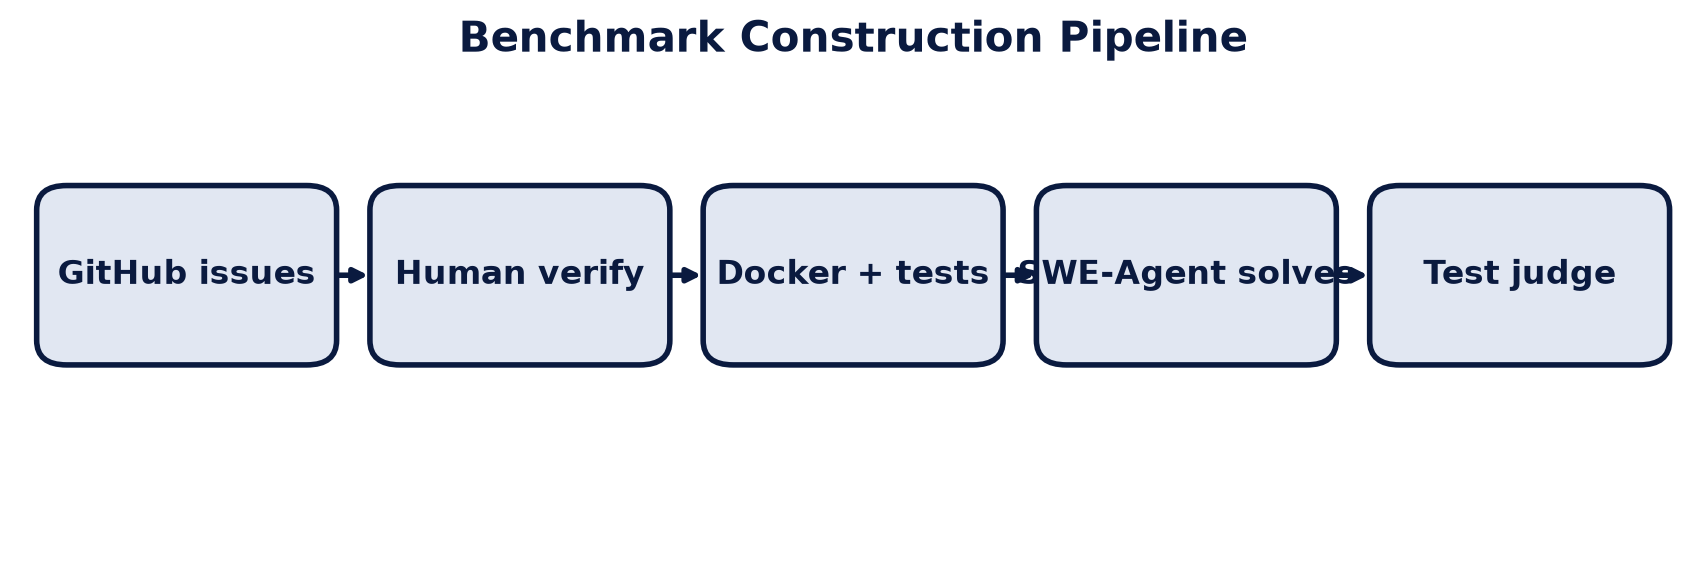
\includegraphics[width=0.9\textwidth,height=0.62\textheight,keepaspectratio]{images/swebenchpro_1.png}
\end{center}
\end{frame}

\section{System Architecture}
\begin{frame}{Evaluation Architecture}
\begin{center}
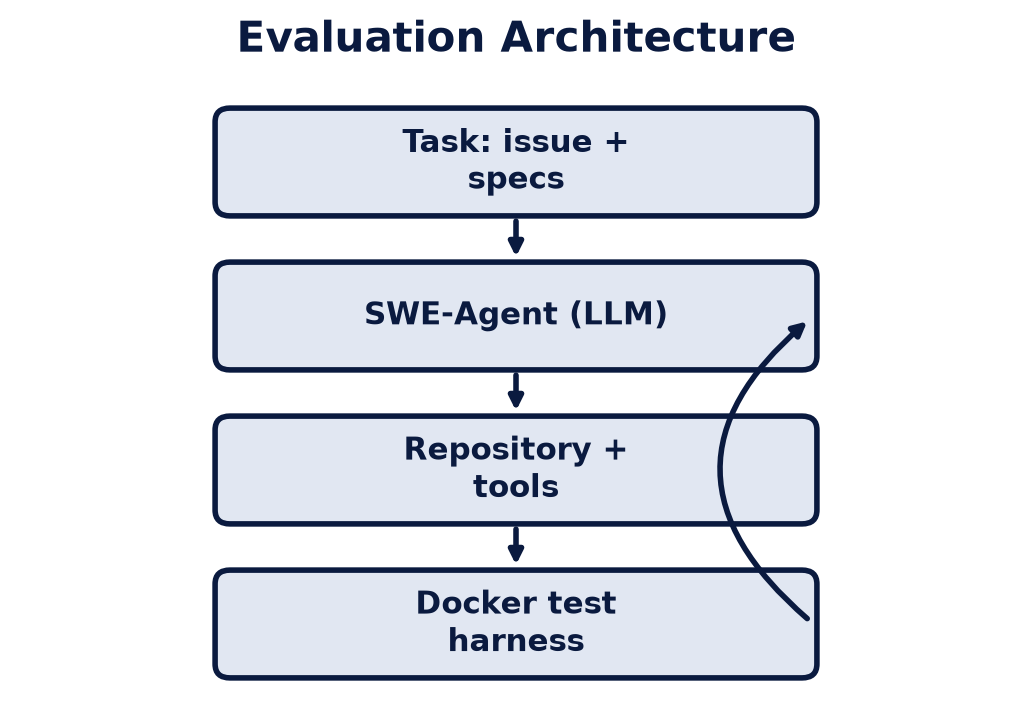
\includegraphics[width=0.9\textwidth,height=0.62\textheight,keepaspectratio]{images/swebenchpro_2.png}
\end{center}
\end{frame}

\begin{frame}{Task Specification}
\begin{itemize}
\item Problem statement: the original issue.
\item Requirements: expected behavior from tests.
\item Interface specs: signatures to avoid false negatives.
\item Verified fail-to-pass and pass-to-pass tests.
\end{itemize}
\end{frame}

\section{Data Collection}
\begin{frame}{Datasets and Repositories}
\begin{itemize}
\item 41 repositories, 1,865 total tasks.
\item Public: 11 GPL repos (731 tasks).
\item Held-out: 12 repos (858 tasks).
\item Commercial: 18 startup repos (276 tasks).
\item Languages: Python, JavaScript, TypeScript, Go.
\end{itemize}
\end{frame}

\section{Model Development}
\begin{frame}{Agent Loop and Judging}
\begin{itemize}
\item SWE-Agent reads, edits, runs tests iteratively.
\item Copyleft (GPL) licenses deter data reuse.
\item Held-out and commercial sets resist overfitting.
\item Tests run thrice; only stable results kept.
\end{itemize}
\end{frame}

\section{Results}
\begin{frame}{Headline Results}
\begin{itemize}
\item Best agents solve only about 23\%.
\item Public set: GPT-5 23.3\%, Opus 4.1 22.7\%.
\item Sonnet 4 17.6\%, Gemini 2.5 Pro 13.5\%.
\item Commercial: Opus 17.8\%, GPT-5 14.9\%.
\end{itemize}
\end{frame}

\begin{frame}{Verified vs.\ Pro: Sharp Drop}
\begin{center}
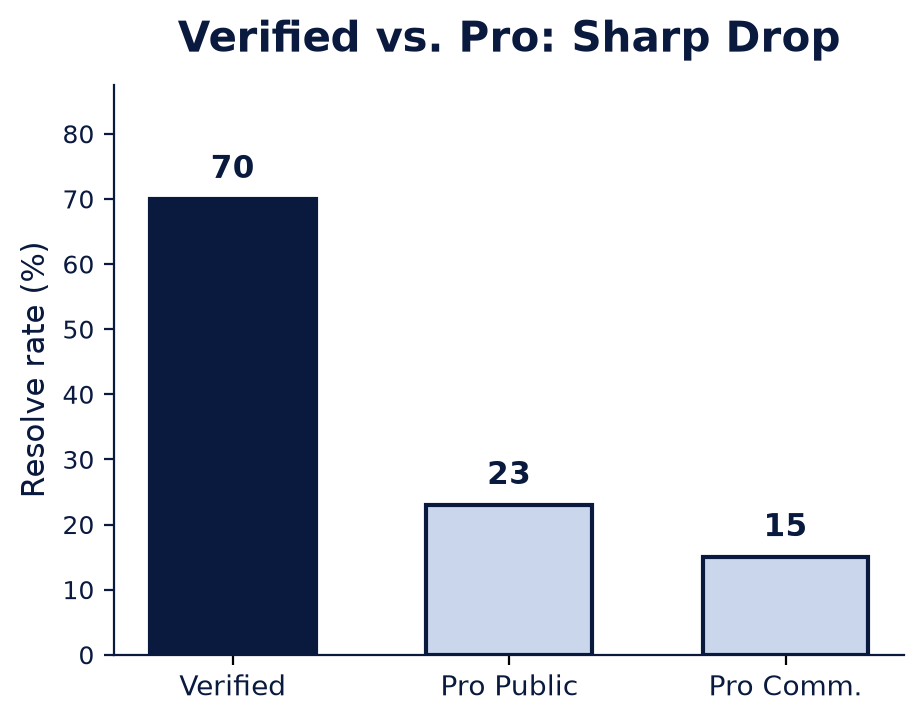
\includegraphics[width=0.9\textwidth,height=0.62\textheight,keepaspectratio]{images/swebenchpro_3.png}
\end{center}
\end{frame}

\section{Discussions}
\begin{frame}{Interpreting the Findings}
\begin{itemize}
\item Public benchmarks overstate real agent ability.
\item Unseen commercial code exposes weak generalization.
\item Long-horizon, multi-file work stays hard.
\item Test-based judging curbs reward hacking.
\end{itemize}
\end{frame}

\section{Challenges}
\begin{frame}{Failure Modes and Limitations}
\textbf{\textit{Six-category failure taxonomy}}
\begin{itemize}
\item Wrong solutions dominate (Opus 4.1 $\approx$ 35.9\%).
\item Small models fail on tool use (Qwen $\approx$ 42\%).
\item Poor localization across many files.
\item Instruction-following, edge-case, syntax errors.
\end{itemize}
\end{frame}

\section{Future Work}
\begin{frame}{Future Directions}
\begin{itemize}
\item Stronger long-horizon planning and memory.
\item Better code localization and tool use.
\item Broaden languages and application domains.
\item Refresh held-out set to track overfitting.
\end{itemize}
\end{frame}

\section{Conclusion}
\begin{frame}{Conclusion}
\begin{itemize}
\item SWE-Bench Pro: 1,865 hard, verified tasks.
\item Contamination-resistant, multi-file, long-horizon.
\item Frontier agents solve only about one in four.
\item Failure taxonomy charts the road ahead.
\end{itemize}
\end{frame}

\section{References}
\begin{frame}{References}
\footnotesize
\begin{itemize}
\item X. Deng, J. Da, E. Pan, et al., ``SWE-Bench Pro: Can AI Agents Solve Long-Horizon Software Engineering Tasks?,'' arXiv:2509.16941, 2025.
\item C. E. Jimenez, J. Yang, A. Wettig, et al., ``SWE-bench: Can Language Models Resolve Real-World GitHub Issues?,'' in Proc. ICLR, 2024.
\item J. Yang, C. E. Jimenez, A. Wettig, et al., ``SWE-agent: Agent-Computer Interfaces Enable Automated Software Engineering,'' in Proc. NeurIPS, 2024.
\end{itemize}
\end{frame}
\begin{frame}\vfill\centering{\Huge Thank You}\vfill\end{frame}
\end{document}
